\documentclass[10pt,norsk,a4paper]{article}
\usepackage[utf8]{inputenc}
\usepackage[T1]{fontenc}
\usepackage[norsk]{babel}
\usepackage[cm]{fullpage}
\usepackage{color}
\usepackage{parskip,textcomp,amssymb,graphicx}
\usepackage{pdfpages}
\usepackage[stable]{footmisc}
\usepackage{multicol}


\title{Generalforsamling \\
	Våren 2018\\[3cm]
	
\includegraphics[width=0.5\textwidth]{cyb-logo.eps}\\[-.5cm]}
\date{2.\ mai 2018}
\author{Cybernetisk Selskab}

% Blank header, samt footer med side x av y
\usepackage{fancyhdr}
\pagestyle{fancy}
\renewcommand{\headrulewidth}{0pt}
\fancyhead{}
\cfoot{Side~\thepage\ av~\pageref{lastpage}}



\begin{document}

\maketitle{}
\newpage
\tableofcontents{}


\section{Valg av møteleder}

\section{Valg av referent}

\section{Valg av protokollunderskrivere}

\section{Valg av tellekorps}

\section{Godkjenning av innkalling}

\section{Godkjenning av dagsorden}

\section{Semesterberetninger}
\subsection{Semesterberetning ved leder}
\textit{\small Korrigert etter utsendt dagsorden.}

\textit{Kjære interne, medlemmer og studenter,}
\begin{multicols}{2}

	% TODO Fyll inn, Andreas
	Her går teksten...

\end{multicols}
% TODO Hilsen her, Andreas

\textbf{Andreas Hansen},\\
leder \\
\date{2.\ mai 2018}
\newpage


\subsection{Semesterberetning ved kjellermogul}

\begin{multicols}{2}
Semesteret startet med et positivt smell, hvor vi fikk både nytt kassesystem og en oppgradering av tappeanlegget. Oppgraderingen av tappeanlegget førte til en del problemer i starten, men etter en del frem og tilbake med tekniker fra Aass så ble mer eller mindre alle problemene løst. Aass har nå fått seg en teknikker som jobber fast i Oslo, noe som har gitt oss en del bedre oppfølging og vedlikehold gjennom semesteret. Det nye kassasystemet viste seg derimot å bli et større problem. Her har vi brukt mye tid på å få svar fra Ajour, men ikke til noe særlig nytte. Slik det er nå fungerer ikke integrasjonen mot tripletex, og det er diverse andre problemer som ikke lar seg fikse uten videre. Grunnet dette ga KS Fredrik Magnussen et mandat til å jakte på et nytt og bedre system. Det viser seg at det ikke bare er vi som sliter, og har nå fått med oss RF, Kjelleren og Uglebo på saken. Forhåpentligvis finner vi et nytt og mer robust system.\\

Forholdsvis tidlig i semesteret ble vi kontaktet av HansaBorg, som ønsket at vi skulle bytte til dem. Etter et positivt møte med en salgsperson fra dem fikk vi omsider er knakende bra tilbud. Siden vi føler såpass mye tilhørighet til Aass, kontakter Tor-Aksel vår kontakt, som ønsket et møte så kjapt som dagen derpå. Utfallet av dette møtet gikk over all forventning, og førte til en avtale som gir oss mange økonomiske fordeler med mer. Blant annet fikk vi endelig lov til å ha et “aktivitetstårn”, som teknikeren fra Aass monterte knappe uken etter at avtalen var signert.\\

Videre har undertegnede sendt inn en søknad til Sparebankstiftelsen DNB, hvor vi søker om 80 000 til en ny espressomaskin. Som med mesteparten av utstyret i Escape begynner også denne å synge på siste verset. Derfor kommer vi forhåpentligvis til å bytte denne ut ila neste semester. Ellers har det vært små reperasjoner på alt fra oppvaskmaskin til kjøleskap. Den siste av kaffetrakterene ble også byttet ut da den eldste av dem sviktet.\\

For å gjøre Escape litt mer koselig har det blitt kjøpt inn noe nytt inventar. Det ble blant annet kjøpt inn to nye hyller; en stor til brettspillene, og en litt mindre som skal fylles med bøker fra realfagsbiblioteket. Som vi forøvrig er i samtale om å få et offisielt samarbeid med. Det har også blitt kjøpt inn noen “planter” for å spice opp lokalet litt.\\

Torsdagsklubben er som forrige semester noe vi har fortsatt med. Det har vært litt varierende kvalitet på arrangementene, og dermed har også deltagelsen vært varierende. Men det har vært en positiv erfaring å ha med seg, da flere funker får opplæring i noe litt utenom tapping av øl. I den sammenheng har det også blitt utarbeidet en liten “standardmeny” for spritholdige drinker. Forhåpentligvis er Torsdagsklubben noe som vil plante seg blant klientellet som et fast tilbud, hvor oppmøtet på sikt, forhåpentligvis, vil øke. Ellers har det vært svært høy aktivitet i Escape, hvor det har vært arrangert alt fra brettspill til et stort antall utlån.\\

En ting som har vært litt problematisk dette semesteret for driften av Escape, er internmassen. Vi har rett og slett ikke vært flinke nok til å rekruttere dette semesteret, og det har ført til at få folk har jobbet veldig mye. Selvsagt er det positivt at vi har såpass flinke og engasjerte interne, men det kunne gjerne ha vært fler.\\

Alt i alt har dette semesteret gått rundt som vanlig, med en del små og store forandringer. Internt i KS kunne kommunikasjonen vært litt bedre. Dette er forhåpentligvis noe de som sitter videre, og de nye som kommer inn kan jobbe sammen om for å forbedre. Videre er det noen ting som burde bli gjort neste semester:\\
\begin{itemize}
		\item Rekruttere bedre i starten av semesteret (studiestartuka er en gullgruve)
		\item Finne en bedre kasse, om mulig
		\item Bedre oppfølging av rutiner
		\item Bedre intern kommunikasjon
\end{itemize}
\end{multicols}
Vi sees i Escape!

\textbf{Adrian Helle}, \\
kjellermogul \\
\date{24.\ april 2018}

%\newpage

\section{Kasserer orienterer}
\subsection{Regnskapets tilstand}
Kasserer presenterer regnskapet.


\subsection{Revidert budsjett for høsten 2018}
Kasserer presenterer budsjett.


\section{Kontigentfastsettelse}
Hovedstyret foreslår å holde medlemskontigenten kr. 40,-.

\section{Vedtektsendring: forslag til endring av stemmemetodikk}

\section{Valg}

\begin{minipage}[t]{0.49\textwidth}
\subsection{Hovedstyret} %TODO Oppdater listen med verv
Man velges inn i hovedstyret for ett år av gangen.

\subsubsection{Leder}
\subsubsection{Nestleder}
\subsubsection{Arrangementssjef}
\subsubsection{Rekrutteringsanasvarlig}

\end{minipage}
\begin{minipage}[t]{0.49\textwidth}
\subsection{Kjellerstyret} %TODO Oppdater listen med verv
Alle verv som er til valg i kjellerstyret gjelder for ett semester av gangen.

\subsubsection{Innkjøpsansvarlig}
\subsubsection{Barsjef}
\subsubsection{Kafésjef}
\subsubsection{Teknisk ansvarlig}
\subsubsection{DJ-sjef}
\subsubsection{Utlånsansvarlig}
\subsubsection{Arrangementskoordinator}

\end{minipage}

\newpage

\section{Vedtektsendringer}
Følgende forslag til vedtektsendringer ligger fremme.

\subsection{Endring i forbindelse med krav om Ifi-foreninger}

For å være en offisiell Ifi-forening har Ifi satt sammen noen vedtekter som studentforeningene må følge.
Per dags dato følger ikke Cybernetisk Selskab §1c\footnotemark. Det ble lagt frem et forslag av hovedstyret på vårens generalforsamling om å endre våre vedtekter, slik at vi ikke bryter med Ifi sine krav.
Dette ble da ikke vedtatt da forsamlingen konkludere med at de nye vedtektene var for åpne og uklare. Forsamlingen ønsket at hovedstyret skulle komme med et nytt forslag til neste generalforsamling, som blir denne, høsten 2017.

\footnotetext{Etter manglende vedtektsfesting av to-tredelers Ifi-studenter i hovedstyret.}

Om vedtektene ikke blir vedtatt vil hovedstyret starte søknadsprosessen for å få et unntak fra §1c av \textit{Vedtekter for Ifi-forening}, slik som §3c åpner for. Begge endringsforslagene hører sammen og stemmes over i lag.

Hovedstyret er innstilt på å starte søknadsprosessen etter §3c.

\subsubsection{Forslag til ny paragraf: §5h}
\begin{quote}
	\begin{enumerate}
		\item[§5h] Minimum to-tredeler av hovedstyret skal bestå av studenter som enten (1) er tilknyttet et eller flere studieprogrammer ved \textit{Institutt for informatikk}, eller (2) som tar ett eller flere IN- eller INF-fag.
	\end{enumerate}
\end{quote}

\subsubsection{Forslag til endring av paragraf: §8a}
\begin{quote}
	\begin{enumerate}
		\item[§8a]
			Valgbare til alle styrer er alle medlemmer i henhold til §2 og informatikkstudenter ved Universitetet i Oslo. \textcolor{red}{Om valg av kandidat bryter med §5h, blir valget gjort ugyldig og det blir gjenvalg. Om ingen andre kandidater stiller blir vervet etterfylt av hovedstyret i henhold til §5f.} Alle valg avgjøres \textcolor{red}{på generalforsamling} ved simpelt flertall.
	\end{enumerate}
\end{quote}


\section{Æresmedlemskap}

\section{Utdeling av pins}

Arkivar deler ut pins.

\section{CYB50}

CYB har 50 års jubileum februar 2019, og trenger i den sammenheng frivillige til dette formålet. Leder for komitèen orienterer litt om planer sålangt.

Interesse for deltagelse i arrangeringen kan sendes til \textbf{cyb50@cyb.no}

\section*{Vedlegg: Cybernetisk Selskabs vedtekter}
\section*{Vedlegg: Vedtekter for Ifi-foreninger}\label{lastpage}


\newpage

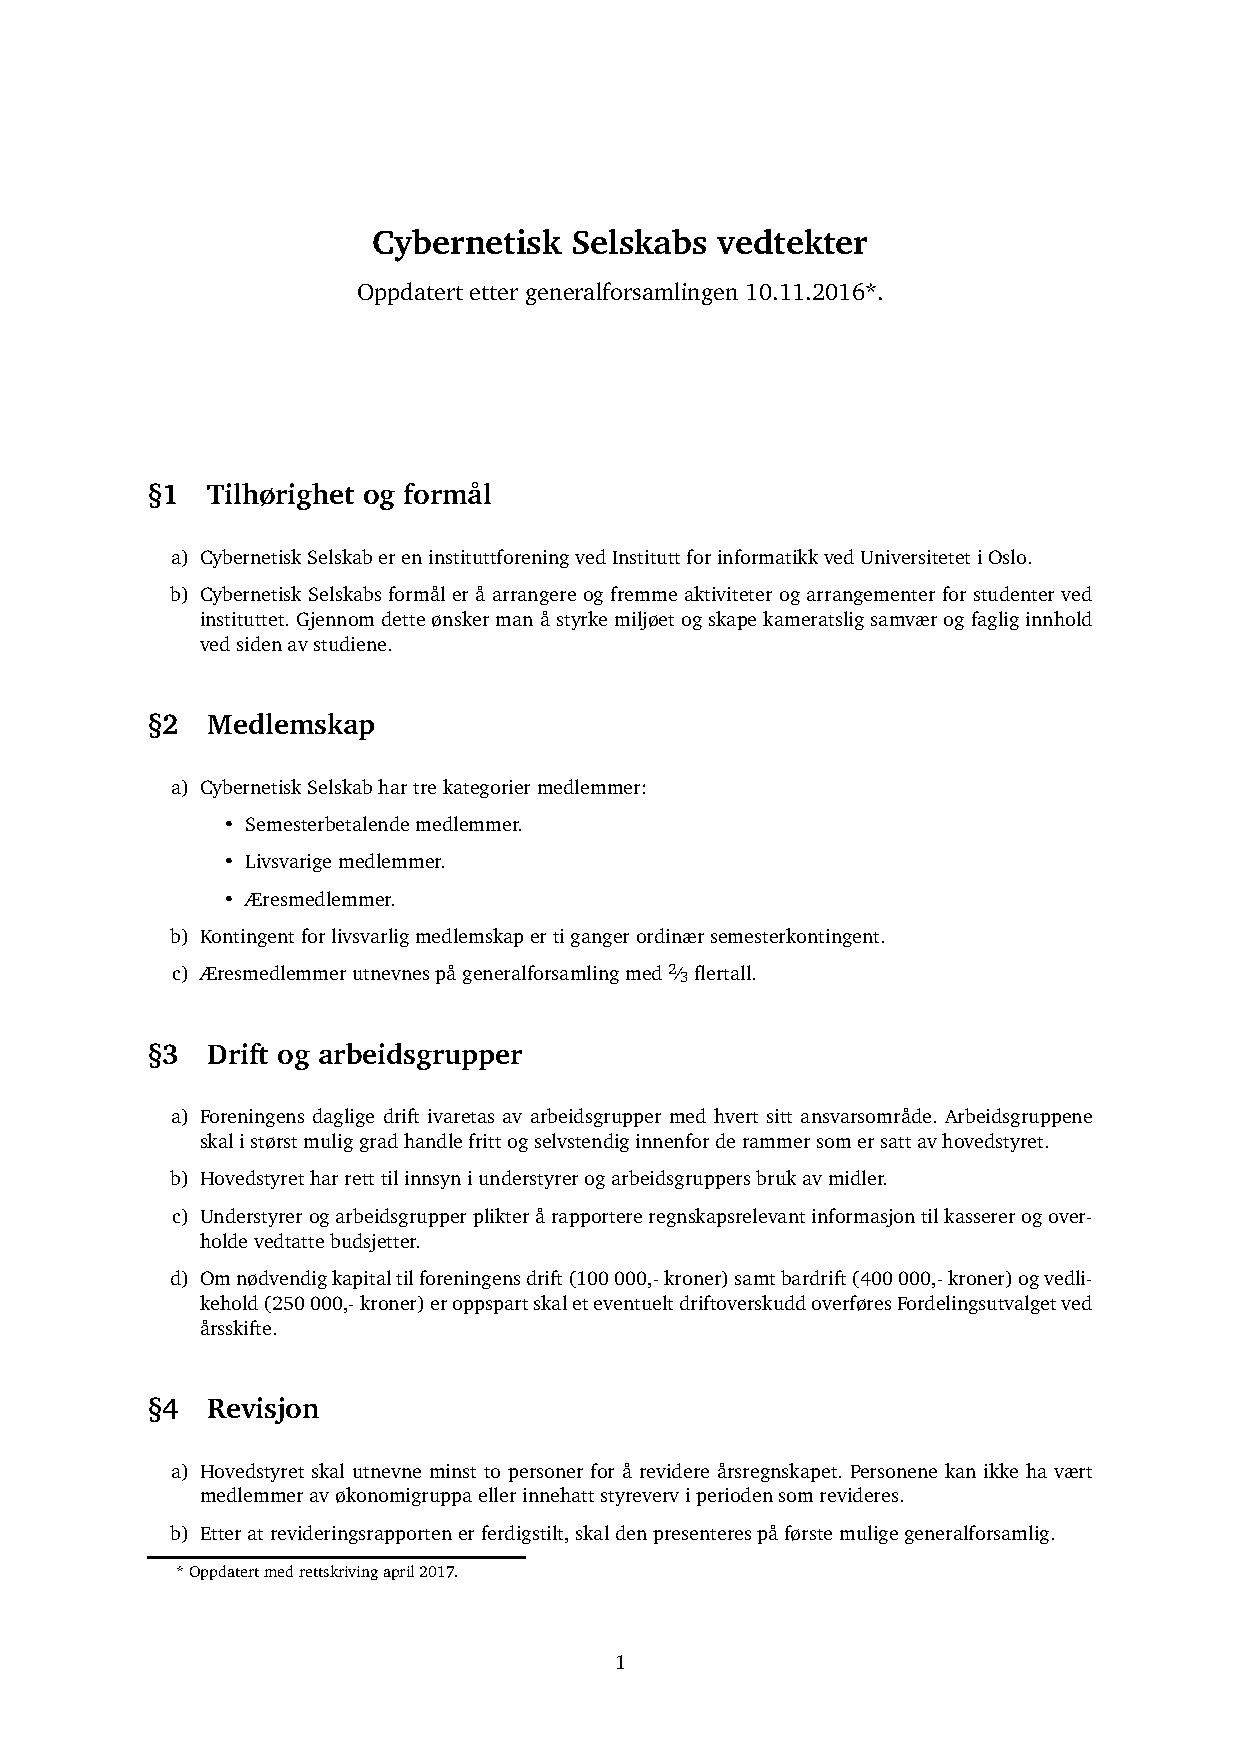
\includepdf[pages=-]{cyb-vedtekter.pdf}
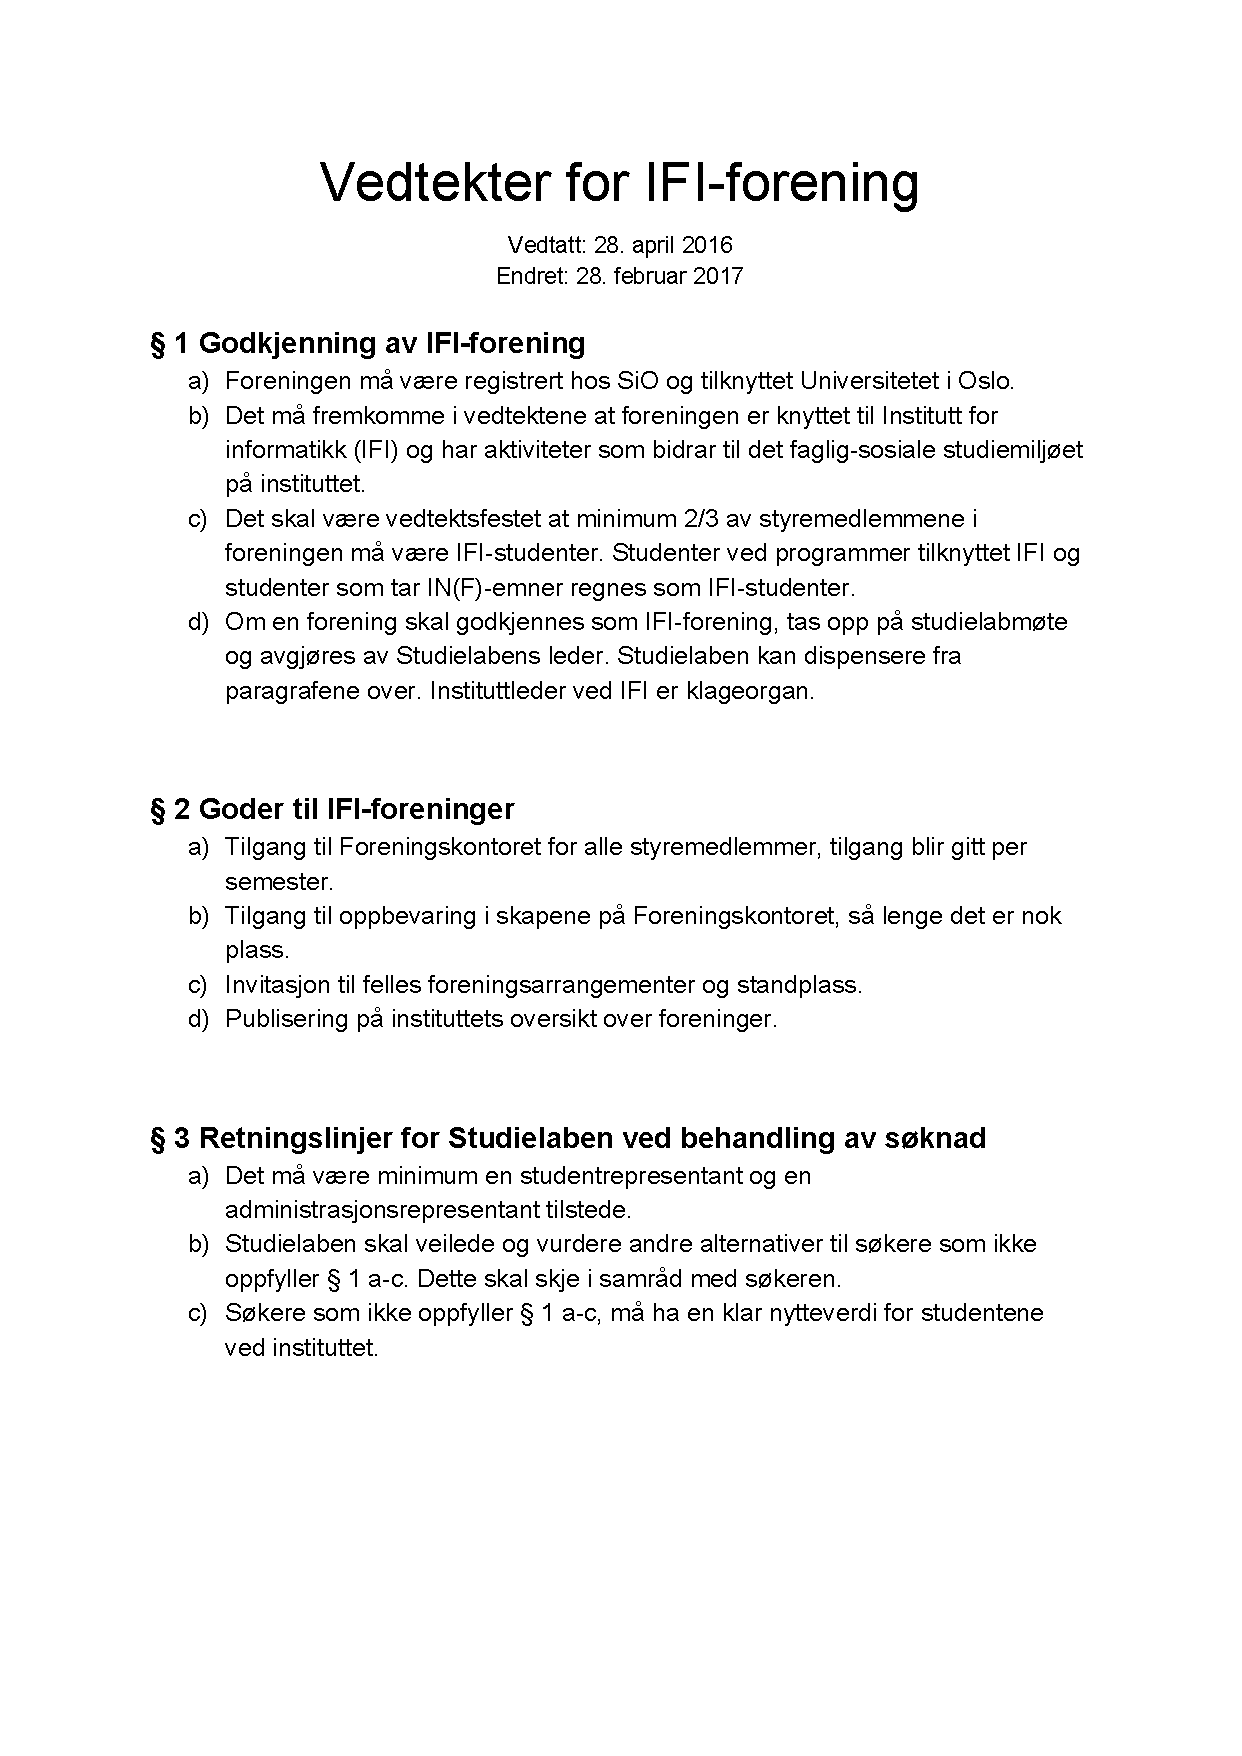
\includepdf[pages=-]{ifi_forening_vedtekter_2017.pdf}
\end{document}
